% !TEX root = main.tex
\subsection{Optimism-only fails to learn classification decisions (Proposition~\ref{prop:fail-to-learn})}\label{app:fail-to-learn}
This appendix gives the proof of Proposition~\ref{prop:fail-to-learn} in Appendix~\ref{app:prop-fail-to-learn}. In Appendix~\ref{app:sim-fail-to-learn}, we simulate several alternatives of $\textsc{BACID.UCB}$ using a setting similar to the example in Proposition~\ref{prop:fail-to-learn}. We observe that these alternatives either fail to learn classification decisions, or incur much higher loss, supporting the robustness of our observation in Proposition~\ref{prop:fail-to-learn} and the efficiency of our algorithm.

\subsubsection{Proof of Proposition~\ref{prop:fail-to-learn}}\label{app:prop-fail-to-learn}
We recall the setting. There are two types ($K = 2$) and the cost distributions for each type are
\[
\set{F}_1 = \{\pm 1~\text{with probability 0.5}\}, \set{F}_2 = \{-0.01~\text{with probability 0.05};~+0.01~\text{with probability 0.95}\}.
\]
The algorithm is run with exact knowledge of $\set{F}_1$ and with  knowledge that $\ell_2 \leq 0.01$. We assume the algorithm sets $\bar{\ell}_2(t) \leq 0.01$ as a result. Arrival rates are such that $\lambda_1(t) = 1,\lambda_2(t) = 0$ for $t \leq T_1 \coloneqq \lfloor \frac{\beta}{2} \rfloor$, and $\lambda_1(t) = 5/6, \lambda_2(t) = 1/6$ for $T_1 < t \leq T$. The service rate is $\mu_1 = \mu_2 = 1/2$ with $N(t) = 1$ for any $t$. We know that $\ell_2^+ - \ell_2^- = (0.95 - 0.05)0.01 > 0$, meaning that wrongly accepting a type-$2$ job incurs a constant positive loss. We define $Q_{\max} = \ell_1\beta = 0.5\beta$. 

\begin{lemma}\label{lem:bound-q2}
For any period $t$, the number of type-2 jobs admitted for review is $Q_2(t) < \frac{Q_{\max}}{25}$.
\end{lemma}
\begin{proof}
It holds that $\ell_1 = \min(\ell_1^+, \ell_1^-) = 0.5$. In addition, the admission rule is that $A(t) = 1$ if $\beta \bar{\ell}_{\kappa(t)}(t) > Q_{\kappa(t)}(t)$. Since we assume the algorithm sets $\bar{\ell}_2(t) \leq 0.01$, it holds that the algorithm admits a type-$2$ job only if
$Q_2(t) \leq \beta / 100$, which, by the same analysis in the proof of Lemma~\ref{lem:known-delay}, implies that $Q_2(t) \leq \beta /100 + 1 < \frac{Q_{\max}}{25}$, where the last inequality is by $Q_{\max} = 0.5\beta$ and $\beta / 100 + 1 < \beta / 50$ when $\beta > 100$.
\end{proof}
We define the event $\set{E}$ where for all periods $t$ in $[T_1,T]$, we have $Q_1(t) \geq \frac{Q_{\max}}{25}$, i.e., $\set{E} = \{\forall t \in [T_1+1,T], Q_1(t) \geq Q_{\max}/25\}$. The following lemma shows event $\set{E}$ happens with high probability.
\begin{lemma}\label{lem:prob-event-e}
With high probability, there are at least $\frac{Q_{\max}}{25}$ type-1 admitted jobs:
$\Pr\{\set{E}\} \geq 1 - 2/T$.
\end{lemma}
\begin{proof}
Our proof strategy is as follows. We first show that by a concentration bound, the queue length of type-$1$ jobs must increase linearly in the interval, given that the queue length is less than $Q_{\max}$ in the entire interval. In this case, for any period $t$, either there is a period $\tau$ with $Q_1(\tau) \geq Q_{\max}$ in the last $Q_{\max}/4$ periods, which implies $Q_1(t) \geq Q_{\max}-Q_{\max}/4$; or $Q_1(\tau)$ grows linearly in the last $Q_{\max}/4$ periods, which also implies $Q_1(t) = \Omega(Q_{\max}).$

Formally, we define $\hat{S}_k(t)$ as the Bernoulli random variable indicating whether the review of a type-$k$ job will finish in this period, given that we schedule such a job. Then $\hat{S}_k(t)$ has mean $N(t)\mu_k=1/2$, and the true review outcome is $S_k(t) = \hat{S}_k(t)\psi_k(t)$. 
We denote $E = \lceil Q_{\max} / 4\rceil$. For $t > T_1 > E$, we define 
\[
\tilde{\set{E}}_t = \left\{\sum_{\tau= t - E}^{t-1} \Lambda_1(\tau) \geq \frac{5E}{6} - \sqrt{E\ln T}\right\} \cap \left\{\sum_{\tau= t - E}^{t-1} \hat{S}_1(t) \leq \frac{E}{2} + \sqrt{E\ln T}\right\}.
\]
By Hoeffding Inequality and union bound, we have $\Pr\{\tilde{\set{E}}_t\} \geq 1 - 2/T^2$ since $\expect{\Lambda_1(t)} \geq \frac{5}{6}$. We define $\tilde{\set{E}} = \cap_{t > T_1}\{\tilde{\set{E}}_t\}$. By union bound, we have $\Pr\{\tilde{\set{E}}\} \geq 1 - 2/T$. It remains to show that under $\tilde{\set{E}}$, it holds that $Q_1(t) \geq \frac{Q_{\max}}{25}$ for any $t > T_1$, and thus $\Pr\{\set{E}\} \geq \Pr\{\tilde{\set{E}}\} \geq 1 - 2/T.$

We fix a period $t > T_1$ and look at the interval $[t - E,t - 1]$. Since $Q_{\max} = 0.5\beta \geq 25$, it holds that $E < Q_{\max} / 2$. We consider two cases:
\begin{itemize}
\item there exists $\tau \in [t-E,t-1]$ such that $Q_1(\tau) \geq Q_{\max}$. In this case, it holds that \[Q_1(t) \geq Q_1(\tau) - (t-\tau) \geq Q_1(\tau) - E \geq Q_{\max} - E \geq Q_{\max} / 2\]
where the first inequality is because at most one type-$1$ job is reviewed per period.
\item for every $\tau \in [t-E,t-1]$, it holds that $Q_1(\tau) < Q_{\max}$. The admission rule and the assumption that $\set{F}_1$ is known perfectly imply that $A(\tau) = \indic{0.5\beta > Q_1(\tau)} = 1$ for every $\tau \in [t-E,t-1]$ with $\kappa(\tau) = 1$. As a result, conditioning on $\tilde{\set{E}}$,
\begin{align*}
Q_1(t) &\geq Q_1(t-E)+\sum_{\tau=t-E}^{t-1} \indic{\kappa(\tau)=1}A(\tau) - \sum_{\tau=t-E}^{t-1} \hat{S}_1(\tau) = \sum_{\tau=t-E}^{t-1} \Lambda_1(\tau) - \sum_{\tau=t-E}^{t-1} \hat{S}_1(\tau) \\
&\geq \frac{5E}{6} - \sqrt{E\ln T} - \frac{E}{2} - \sqrt{E\ln T} = \frac{E}{3}-2\sqrt{E\ln T} \overset{(a)}{\geq} \frac{E}{6} \geq \frac{Q_{\max}}{25},
\end{align*}
where (a) is because $T \leq \exp(Q_{\max} / 576) \leq \exp(E / 144)$.
\end{itemize}
Combining the above discussions then shows that, conditioning on $\tilde{\set{E}}$, it holds that $Q_1(t) \geq Q_{\max} / 25$, which finishes the proof.
\end{proof}

\begin{proof}[Proof of Proposition~\ref{prop:fail-to-learn}]
Let us condition on $\set{E}$, which happens with probability at least $1 - 2/T$ by Lemma~\ref{lem:prob-event-e}. Since the algorithm follows the scheduling rule that prioritizes the review of the type with the larger $\mu_k Q_k(t)$ in every period, it is guaranteed that only type-$1$ jobs get reviewed after $T_1$ because $\mu_1 = \mu_2$ and $Q_1(t) \geq \frac{Q_{\max}}{25} > Q_2(t)$ where the last inequality is by Lemma~\ref{lem:bound-q2}. But type-$2$ jobs only arrive after $T_1$. As a result, there is no review for type-$2$ jobs.
\end{proof}

\subsubsection{The failure of other exploration heuristics}\label{app:sim-fail-to-learn}
Although Proposition~\ref{prop:fail-to-learn} assumes a particular form of optimism-only approaches ($\textsc{BACID.UCB}$), this section simulates several alternatives and finds that they either still fail to learn correct classification or incur much higher loss than $\bacidol$. 
Similar to Proposition~\ref{prop:fail-to-learn}, we consider a setting with two types. Type-$1$ jobs have costs $+1$ with probability $0.49$ and costs $-1$ with probability $0.51$. Type-$2$ jobs have costs $+1$ with probability $0.3$ and costs $-0.3$ with probability $0.7$. Their arrival rates are $\lambda_1(t) = 0.5, \lambda_2(t) \equiv 0.5$. We set $\mu_1 = 0.4, \mu_2 = 0.1$ and $N(t)=1$. The time horizon is $T = 10^5$. With perfect knowledge of the cost distributions, the optimal classification decisions are to accept all type-1 jobs but reject all type-2 jobs. The algorithm should admit all type-$1$ jobs but zero type-$2$ jobs for human reviews. We simulate three variants of $\textsc{BACID.UCB}$: 
\begin{itemize}
\item Loss-weighted $\textsc{BACID.UCB}$: this algorithm  follows the same classification and admission decisions as $\textsc{BACID.UCB}$ in Section~\ref{sec:opti-fail}, but schedules a type-$k$ job with $k$ that maximizes $\bar{\ell}_k(t)\mu_k Q_k(t).$ That is, its prioritization rule also incorporates the optimistic estimate $\bar{\ell}_k(t)$. This may help prioritize the job type with higher uncertainty in the unknown loss $\ell_k.$ 
\item $\textsc{BACID}$ with discounted UCB: a potential approach to encourage exploration is to use a time-based exploration bonus. We consider a variant of the above loss-weighted $\textsc{BACID.UCB}$. For the admission decision  that checks whether $\beta \bar{\ell}_{\kappa(t)}(t)\geq Q_{\kappa(t)}(t)$, we modify the confidence bound estimate of $\bar{\ell}_{\kappa(t)}(t)$. Instead of following \eqref{eq:conf-r}, we discount samples collected in period $s$ by $(0.99)^{t-s}$ for the confidence bound in period $t$. Hence, the further a type of job was reviewed, the larger confidence bound this type will obtain. This discounted UCB approach was used in \cite{Avadhanula2022} to handle non-stationarity in cost distributions, but our purpose here is to understand whether it can bring sufficient exploration for classification decisions. 
\item $\textsc{InitExplore}$: this algorithm adds an initial exploration phase to $\textsc{BACID.UCB}$. Specifically, in the first $T_1 = T^{2/3}\ln(T)^{1/3}$ periods, it admits all jobs into the human review queue and schedules either type of jobs for review with equal probability. After the first $T_1$ exploration periods, the algorithm follows $\textsc{BACID.UCB}.$ We set $T_1$ according to the optimal exploration length for explore-then-commit policies in multi-armed bandits (see page 16 of \cite{slivkins2019introduction}).
\end{itemize}
We also simulate $\bacidol$, which uses label-driven admission on top of $\textsc{BACID.UCB}$ to enable fast learning of classification). We take $\gamma = (T/(2\ln (T)))^{-1/3}$ as per Algorithm~\ref{algo:bacidol}. For all $\bacid$-based approach, we take $\beta = \sqrt{T / 2}$. The  confidence bounds are set according to \eqref{eq:conf-h} and \eqref{eq:conf-r} without including the constants.

Our results contain $1000$ independent runs of the above environment. Recall that the algorithm rejects a type-2 job when its \emph{empirical mean} $\hat{c}_2(t)$ is positive for a period $t$. Let $\hat{c}_2(t,i)$ be this estimate for a run $i \leq 1000$. To understand how good the classification decisions are, for every period $t$ we count the percentage of runs with $\hat{c}_2(t,i) \leq 0$, i.e., the (ensemble-average) probability that this optimism-only approach will \emph{wrongly accept} a type-$2$ job for period $t$.

\begin{center}
\begin{minipage}[c]{0.45\textwidth}
  \centering
  
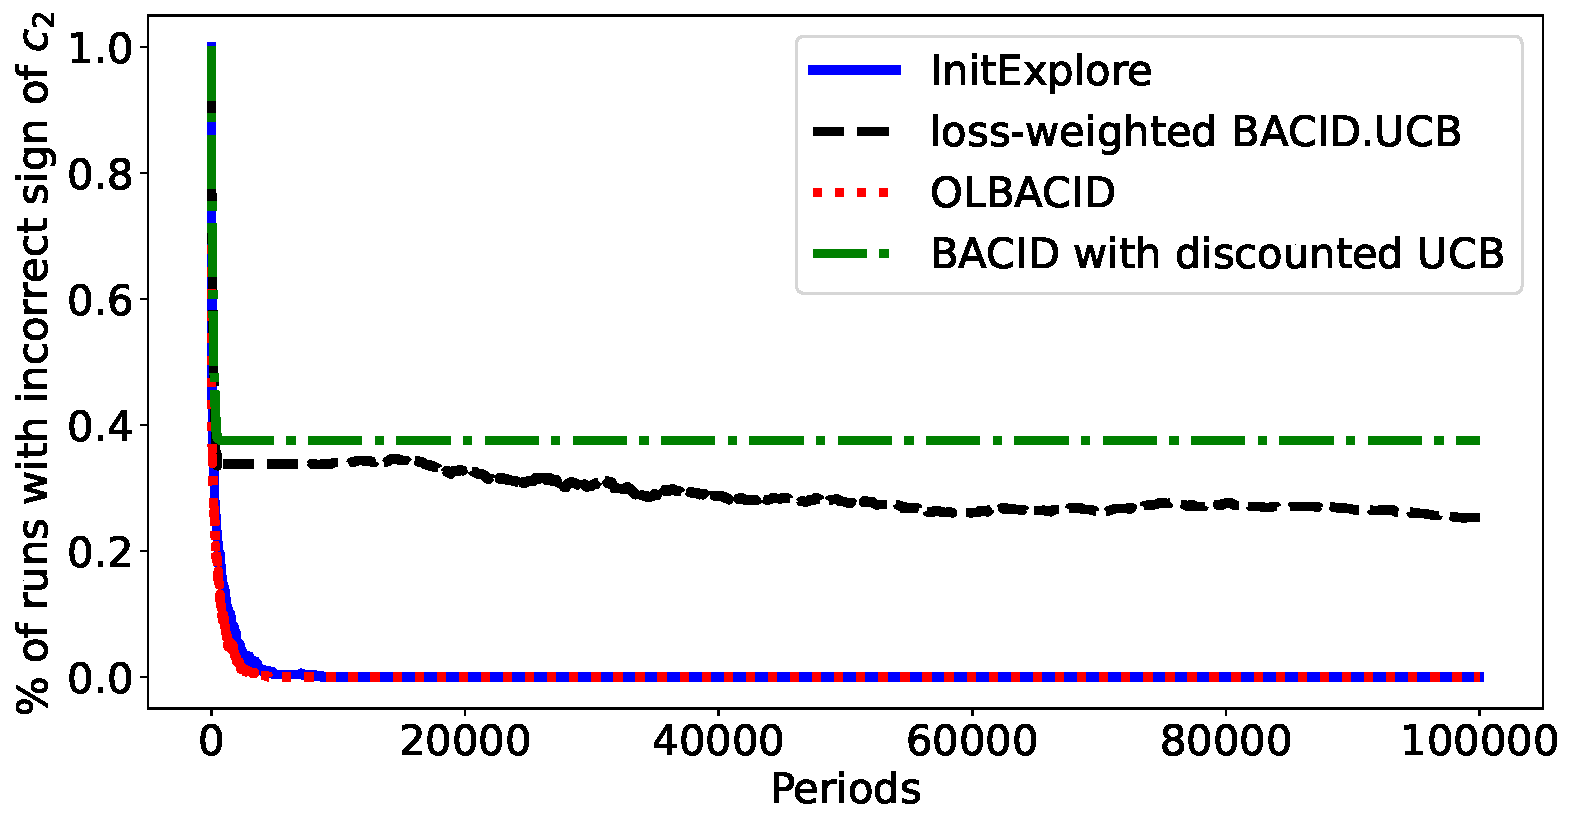
\includegraphics[width=3in]{figures/fail-to-learn.pdf}
  \captionof{figure}{Percentages of runs  in which an algorithm has an estimate $\hat{c}_2(t)$ with wrong signs for period $t$.}
    \label{fig:fail-to-learn}
\end{minipage}
\hspace{0.05\textwidth}
\begin{minipage}[c]{0.45\textwidth}
  \centering
  \begin{tabular}{|c|c|}
\hline
Algorithm                          & Average loss \\ \hline
Loss-weighted $\textsc{BACID.UCB}$ & $8375$                        \\ \hline
$\bacid$ with discounted UCB       & $8552$                        \\ \hline
$\textsc{InitExplore}$             & $9488$                        \\ \hline
$\bacidol$                         & $8148$                        \\ \hline
\end{tabular}
  \captionof{table}{Loss \eqref{eq:policy-loss} of algorithms averaged over $1000$ runs}
  \label{tab:mytable}
\end{minipage}
\end{center}

Figure~\ref{fig:fail-to-learn} shows the results. We observe that for the entire horizon, the optimism-only algorithms (loss-weighted $\textsc{BACID.UCB}$ and $\textsc{BACID}$ with discounted UCB) wrongly accept type-$2$ jobs for at least $20\%$ of the runs. This high failure probability indicates that the algorithm cannot (efficiently) learn how to classify type-$2$ jobs. What seems surprising is that $\textsc{BACID}$ with discounted UCB  may indeed lead to even fewer samples for type-$2$ than the non-discounted version (the former has a higher error probability than the latter in Figure~\ref{fig:fail-to-learn}). This happens because even though type 2 now has a larger confidence bound, type 1 also has a larger confidence bound with discounted UCB, which counteracts the incentive to review type 2.

In addition, although $\textsc{InitExplore}$ learns how to classify type-$2$ jobs in Figure~\ref{fig:fail-to-learn}, it incurs a much higher loss (Table~\ref{tab:mytable}) than $\bacidol$ due to its non-adaptive exploration phase. We also note that $\textsc{InitExplore}$ cannot accommodate a non-stationary setting where the arrival rates of types change across time because its exploration phase is limited to early arrivals. Compared to all these variants of $\textsc{BACID.UCB}$, our algorithm, $\bacidol$, learns to reject type-$2$ jobs for the classification decisions very soon and incurs the lowest loss.

This setting illustrates that simple variants of the optimism-only approaches do not ensure the algorithm to learn correct AI classification decisions in an efficient manner. Our algorithm addresses such shortcomings by using label-driven admission and forced scheduling.

\subsection{Regret guarantee for $\bacidol$ (Theorem~\ref{thm:bacidol})}\label{app:thm-bacidol}

\begin{proof}[Proof of Theorem~\ref{thm:bacidol}]
The regret $\reg^{\bacidol}(T)$ is upper bounded by $c_{\max}T$, which is less than the first term when $K \geq T$. Moreover, if $T \leq 2$, \[\reg^{\bacidol}(T) \leq \loss^{\bacidol}(T) \leq 2c_{\max} \lesssim c_{\max}\sqrt{T\ln T}.\] We thus focus on $T \geq 3$, $K \leq T$ and $
\beta = \sqrt{T / (Kc^2_{\max})}, \gamma = (\nicefrac{T}{K\ln T})^{-1/3}$, which is the setting Lemmas~\ref{lem:bacidol-delay},~\ref{lem:bacidol-class} and \ref{lem:bacidol-idio} are applicable.
Omitting dependence on $\sigma_{\max}, \hat{\mu}_{\min}$, constants and applying Lemmas~\ref{lem:bacidol-delay},~\ref{lem:bacidol-class} and \ref{lem:bacidol-idio} to the corresponding terms in \eqref{eq:learning-loss-decompose}, we obtain:
\begin{equation}\label{eq:bound-olbacid}
\begin{aligned}
\expect{\loss^{\bacidol}(T)} - \loss^\star(T) &\lesssim c^2_{\max}\beta K + \gamma\indic{\gamma > \eta} T + \frac{c_{\max}K\ln T}{\max(\eta,\gamma)^2} + T / \beta + Kc_{\max}\sqrt{T\ln T}\\
&\lesssim Kc_{\max}\sqrt{T\ln T} + \min\left(\frac{K\ln T}{\eta^2}, T^{2/3}(K\ln T)^{1/3}\right).
\end{aligned}
\end{equation}
\end{proof}

\subsection{Regret lower bound when cost distributions are unknown (Theorem~\ref{thm:bacidol-lowerbound})}\label{app:thm-bacidol-lowerbound}
The proof is similar to the standard approach of showing regret lower bound in multi-armed bandits. The proof uses Kullback-Leibler divergence (KL-divergence) defined as follows. For a finite sample space $\Omega$ and two of its probability distributions $p,q$, their KL-divergence is $\kl{p}{q} = \sum_{x \in \Omega} p(x)\ln \frac{p(x)}{q(x)}.$ Our proof uses the following properties of the KL-divergence.
\begin{fact}[theorem 2.2 of \cite{slivkins2019introduction}]\label{fact:KL-divergence}
The KL-divergence of distributions $p,q$ satisfies the next properties:
\begin{itemize}
\item chain rule for product distributions: suppose the sample space is a product $\Omega = \Omega_1\times \cdots \times \Omega_n$ and the two distributions satisfy $p = p_1 \times \cdots \times p_n, q = q_1 \times \cdots \times q_n$ with $p_j, q_j$ being distributions on $\Omega_j$. Then $\kl{p}{q} = \sum_{j=1}^n \kl{p_j}{q_j}.$
\item Pinsker's inequality: for any event $A \subseteq \Omega$, $2(p(A)-q(A))^2 \leq \kl{p}{q}.$
\end{itemize}
\end{fact}
\begin{fact}[fact 3 of \cite{freund2023quantifying}]\label{fact:bound-bernoulli}
The KL-divergence of two Bernoulli random variables with mean $g,q$ can be upper bounded by $\frac{(g-q)^2}{q(1-q)}.$
\end{fact}
Throughout, we suppose that for any type $k$, there is a sequence of costs $X_{k,1},X_{k,2},\ldots,X_{k,T}$ sampled i.i.d. from the cost distribution $\set{F}_k$. When humans successfully review a type-$k$ job, they observe the next cost on the cost sequence of type-$k$. This modification does not change the distribution of the original system since costs of type-$k$ jobs are i.i.d. from $\set{F}_k$. Under this modification, the decision of the algorithm in period $t$ must be a function of the types of arrived jobs $\{\kappa(1),\ldots,\kappa(t)\}$, the observed services $\{\set{S}(1),\ldots,\set{S}(t-1)\}$, and the costs of reviewed jobs $\{\{X_{k,i}\}_{i \leq N_k(t)}\}_{k \in \set{K}}$, where we denote $N_k(t)$ by the number of reviewed type-$k$ jobs before period $t$.
\begin{proof}[Proof of Theorem~\ref{thm:bacidol-lowerbound}]
Fix the time horizon $T$ and consider two settings, denoted by settings $(a)$ and $(b)$. In both settings there are two types such that $\lambda_1 = \lambda_2 = 0.5$ and $\mu_1 = \mu_2 = 0.5$ with $N(t) \equiv 1$. Type-1 jobs have costs $\pm 4$, each with probability $0.5$. Type-2 jobs have a setting-dependent distribution $\set{F}_2^{i}$ for $i \in \{(a),(b)\}$. Specifically, setting $i$ has a constant $p_i$ such that type-2 jobs have costs $-1$ with probability $p_{i}$ and costs $+1$ with probability $1-p_i$. We set $p_{(a)} = 0.5(1-\varepsilon)$ and $p_{(b)}=0.5(1+\varepsilon)$ for some $\varepsilon$ that we tune later. For $i \in \{(a),(b)\}$, We use $\expectsub{i}{\cdot}, \Prsub{i}{\cdot}$ to highlight on which setting the expectation and probability is evaluated.

We first calculate the loss of any feasible policy $\pi$ in either setting. For period $t$, let $\Lambda_2^A(t)$ be an indicator such that it is one when there is a type-$2$ job arrival and the policy accepts this job. Similarly, define an indicator $\Lambda_2^R(t)$ which is equal to one when the policy rejects a new type-$2$ job. In addition, let $S_2^A(t)$ indicate whether in period $t$ humans successfully review a type-$2$ job that was initially accepted. Similarly define $S_2^R(t)$ to indicate whether humans successfully review a type-$2$ job that was initially rejected. Let $N_2 = \sum_{t \leq T} S_2(t)$ be the number of reviewed type-$2$ jobs. Then for setting $i$, the expected loss $\expectsub{i}{\set{L}^{\pi}(T)}$ of policy $\pi$ is given by 
\[
2\expectsub{i}{\sum_{t\leq T} (\Lambda_1(t)-S_1(t))} + \expectsub{i}{\sum_{t\leq T} (\Lambda_2^A(t) - S_2^A(t))(1-p_i)} + \expectsub{i}{\sum_{t\leq T} (\Lambda_2^R(t) - S_2^R(t))p_i}, 
\]
where the first term captures that any unreviewed type-$1$ jobs have expected loss $2$; the second term is that any unreviewed type-$2$ jobs that were initially accepted incur expected loss $1 - p_i$ since type-$2$ jobs have costs $+1$ with probability $1-p_i$; the third term means that any unreviewed type-$2$ jobs that were initially rejected incur expected loss $p_i$.

Noting that $\expectsub{i}{\Lambda_1(t)} = 0.5$ for any $t$ and $\expectsub{i}{\sum_{t \leq T}(S_1(t) + S_2^A(t) + S_2^R(t))} \leq T / 2$, 
\begin{align}
\expectsub{i}{\set{L}^{\pi}(T)} &\geq T - \left(T - 2\expectsub{i}{\sum_{t \leq T}( S_2^A(t) + S_2^R(t))}\right) \nonumber\\
&~~+ \expectsub{i}{\sum_{t\leq T} (\Lambda_2^A(t) - S_2^A(t))(1-p_i)} + \expectsub{i}{\sum_{t\leq T} (\Lambda_2^R(t) - S_2^R(t))p_i} \nonumber\\
&\hspace{-1in}= (2-\max(p_i,1-p_i))\expectsub{i}{\sum_{t \leq T} (S_2^A(t) + S_2^R(t))} + (1-p_i)\expectsub{i}{\sum_{t\leq T} \Lambda_2^A(t)} + p_i\expectsub{i}{\sum_{t\leq T} \Lambda_2^R(t)} \nonumber\\
&\hspace{-1in}\geq \expectsub{i}{\sum_{t \leq T} S_2(t) + (1-p_i)\sum_{t\leq T} \Lambda_2^A(t) + p_i\sum_{t\leq T} \Lambda_2^R(t)} \nonumber\\
&\hspace{-1in}= \expectsub{i}{\sum_{t \leq T} S_2(t) + p_i \sum_{t\leq T} \Lambda_2(t) + (1-2p_i)\sum_{t\leq T} \Lambda_2^A(t)}=\frac{p_i T}{2}+\expectsub{i}{\sum_{t \leq T} S_2(t) + (1-2p_i)\sum_{t\leq T} \Lambda_2^A(t)}.
\label{eq:lower-bound-loss}
\end{align}
Denote the total number of reviewed type-$2$ jobs by $N_2 = \sum_{t \leq T} S_2(t)$. Conditioning on $N_2 = n$, in setting $i \in \{(a),(b)\}$, the indicators $\Lambda_2^A(t), \Lambda_2^R(t)$ are random variables of the sample space formed by $\Omega^i = \Omega' \times X^{i}_{2,1} \times \cdots X^{i}_{2,n}$, where  $\Omega'$ denotes the sample space unrelated to type-$2$ jobs' costs and is thus common for setting $(a)$ and $(b)$; for $j \leq n$,  $X^{i}_{2,j}$ denotes the costs of the $j$-th reviewed type-$2$ jobs and has i.i.d. distribution of $\set{F}_2^{i}.$ Using Fact~\ref{fact:KL-divergence}, for any $t \leq T$,
\begin{align*}
2\left|\Prsub{(a)}{\Lambda_2^A(t) = 1 \mid N_2 = n} -\Prsub{(b)}{\Lambda_2^A(t) = 1 \mid N_2 = n} \right|^2 &\leq \kl{\Prsub{(a)}{\cdot \mid N_2 = n}}{\Prsub{(b)}{\cdot \mid N_2 = n}} \\
&\leq \sum_{j=1}^n \kl{\set{F}_2^{(a)}}{\set{F}_2^{(b)}} \leq  \frac{n\varepsilon^2}{(1-\varepsilon)^2/4},
\end{align*}
where the first two inequalities use Fact~\ref{fact:KL-divergence} and the last inequality uses Fact~\ref{fact:bound-bernoulli}. As a result, 
\begin{equation}\label{eq:bound-dist-diff}
\begin{aligned}
|\expectsub{(a)}{\Lambda_2^A(t) \mid N_2 = n} - \expectsub{(b)}{\Lambda_2^A(t) \mid N_2 = n}| &\leq \frac{\sqrt{2n}\varepsilon}{1-\varepsilon}.
\end{aligned}
\end{equation}
For setting $i$, define the \emph{pseudo-loss} $\tilde{L}^i \coloneqq \sum_{t \leq T} S_2(t) + (1-2p_i)\sum_{t\leq T} \Lambda_2^A(t)$, which is the random variable taken expectation on the right hand side of \eqref{eq:lower-bound-loss}. The sum of the pseudo-losses satisfies
\begin{align*}
&~~\expectsub{(a)}{\tilde{L}^{(a)} \mid N_2 = n} + \expectsub{(b)}{\tilde{L}^{(b)} \mid N_2 = n} \\
&= 2n+\varepsilon\sum_{t \leq T} \expectsub{(a)}{\Lambda_2^A(t) \mid N_2 = n}-\varepsilon \sum_{t \leq T} \expectsub{(b)}{\Lambda_2^A(t) \mid N_2 = n}\\
&\geq 2n - \varepsilon \sum_{t \leq T} \left|\expectsub{(a)}{\Lambda_2^A(t) \mid N_2 = n} - \expectsub{(b)}{\Lambda_2^A(t) \mid N_2 = n}\right| \geq 2n - \frac{\sqrt{2n}\varepsilon^2 T}{1-\varepsilon}.
\end{align*}
Letting $\varepsilon = T^{-1/3}$, which is at most $0.25$ by the assumption that $T \geq 64$, the above inequality simplifies to 
$\expectsub{(a)}{\tilde{L}^{(a)} \mid N_2 = n} + \expectsub{(b)}{\tilde{L}^{(b)} \mid N_2 = n} \geq 2n - \frac{4}{3}\sqrt{2n}T^{1/3}$. The right hand side is minimized when $n = \frac{2}{9}\cdot T^{2/3}$. Therefore,
\[
\expectsub{(a)}{\tilde{L}^{(a)}} + \expectsub{(b)}{\tilde{L}^{(b)}} \geq \min_{n} \left(\expectsub{(a)}{\tilde{L}^{(a)} \mid N_2 = n} + \expectsub{(b)}{\tilde{L}^{(b)} \mid N_2 = n}\right) \geq -\frac{4}{9}T^{2/3}.
\]
Plugging this bound into \eqref{eq:lower-bound-loss} gives
\[
\expectsub{(a)}{\set{L}^{\pi}(T)} + \expectsub{(b)}{\set{L}^{\pi}(T)} = \frac{T}{2} + \expectsub{(a)}{\tilde{L}^{(a)}} + \expectsub{(b)}{\tilde{L}^{(b)}} \geq \frac{T}{2} - \frac{4}{9}\cdot T^{2/3}.
\]
The optimal fluid benchmark of \eqref{eq:fluid} gives $\set{L}^\star(T) = \lambda_2\min(p_i,1-p_i)T = 0.25(1-\varepsilon)T$ for both settings. Therefore,
\begin{align*}
\max\left(\expectsub{(a)}{\set{L}^{\pi}(T)}, \expectsub{(b)}{\set{L}^{\pi}(T)}\right) - \set{L}^\star(T) &\geq \frac{\expectsub{(a)}{\set{L}^{\pi}(T)} + \expectsub{(b)}{\set{L}^{\pi}(T)}}{2} - \set{L}^\star(T) \\
&\hspace{-1in}\geq \frac{T}{4} - \frac{2 T^{2/3}}{9} - \frac{T(1-\varepsilon)}{4} \geq \frac{T^{2/3}}{4} - \frac{2 T^{2/3}}{9} \geq \frac{T^{2/3}}{36}.
\end{align*}
We have thus shown that for any feasible policy $\pi$, there exists a setting (either $(a)$ or $(b)$) in which the policy incurs $\Omega(T^{2/3})$ regret.
\end{proof} 

\subsection{Number of jobs admitted to label-driven queue (Lemma~\ref{lem:connect-et-qe})}\label{app:lem-connect-et-qe}
\begin{proof}[Proof of Lemma~\ref{lem:connect-et-qe}]
We define $S^{\ld}_k(t) \in \{0,1\}$ to be equal to one if and only if $S_k(t) = 1$ and $Q^{\ld}(t) = 1$, i.e., humans review a type-$k$ job from the label-driven queue (whose length is at most one). This implies that:
$$Q^{\ld}(t+1) - Q^{\ld}(t) = E(t) - \sum_{k \in \set{K}}  S_k^{\ld}(t) = E(t) - \sum_{k \in \set{K}} S_k^{\ld}(t)Q^{\ld}(t).$$ We then define an indicator $\set{I}_{k,t}$ which is equal to $1$ if $\set{Q}^{\ld}(t)$ contains a type-$k$ job. Then conditioning on $Q^{\ld}(t) = 1$, the expectation of $\sum_{k \in \set{K}}S_k^{\ld}(t)$ is lower bounded by
\begin{align}
\expect{\sum_{k \in \set{K}} S_k^{\ld}(t) \mid Q^{\ld}(t) = 1} &= \sum_{k \in \set{K}} \Pr\{\set{I}_{k,t} = 1 | Q^{\ld}(t) = 1\}\expect{S_k^{\ld}(t) \mid Q^{\ld}(t) = 1, \set{I}_{k,t} = 1} \nonumber\\
&= \sum_{k \in \set{K}} \Pr\{\set{I}_{k,t} = 1 | Q^{\ld}(t) = 1\}N_k(t)\mu_k \geq \hat{\mu}_{\min}.\label{eq:lowerbound-service}
\end{align}
The second equality is because $\bacidol$ prioritizes jobs in the label-driven queue (Line~\ref{line:bacidol-prio} in Algorithm~\ref{algo:bacidol}); the last inequality uses $N_k(t)\mu_k \geq \hat{\mu}_{\min}$ and $\sum_{k \in \set{K}} \Pr\{\set{I}_{k,t} = 1 | Q^{\ld}(t) = 1\} = 1$. Therefore,
\[
\expect{Q^{\ld}(t+1) - Q^{\ld}(t)} = \expect{E(t)} - \expect{Q^{\ld}(t)\sum_{k \in \set{K}} S_k^{\ld}(t)} \geq \expect{E(t)} - \hat{\mu}_{\min}\expect{Q^{\ld}(t)}
\]
where we use \eqref{eq:lowerbound-service} for the inequality. Telescoping for $t = 1,\ldots,T$, we obtain $\hat{\mu}_{\min}\sum_{t=1}^T \expect{Q^{\ld}(t)} \leq \expect{\sum_{t=1}^T E(t)}$, which finishes the proof.
\end{proof}

\subsection{Confidence bounds are valid with high probability (Lemma~\ref{lem:prob-good-event})}\label{app:lem-prob-good-event}
We first need the following result that a Lipschitz function of a sub-Gaussian random variable is still sub-Gaussian. 
\begin{lemma}\label{lem:sub-gaussian}
Given a sub-Gaussian random variable $X$ with variance proxy $\sigma^2$ and a $1-$Lipschitz function $f(\cdot)$, the random variable $f(X)$ is sub-Gaussian with variance proxy $2\sigma^2.$
\end{lemma}
\begin{proof}
The proof follows a simplified version of the proof of \cite[Theorem~1]{kontorovich2014concentration}. Define $V = f(X) - \expectsub{X'}{f(X')}$ where $X'$ is an independent copy of $X$. By definition, showing that $f(X)$ is sub-Gaussian with variance proxy $2\sigma^2$ is equivalent to showing that $\expectsub{X}{\exp(sV)} \leq \exp(s^2(2\sigma^2)/2)$ for any $s \in \mathbb{R}.$ Fixing $s \in \mathbb{R}$ and expanding the term gives
\begin{align*}
\expectsub{X}{e^{sV}} &= \expectsub{X}{e^{s\expectsub{X'}{f(X)-f(X')}}} \\
&\leq \expectsub{X,X'}{e^{s(f(X)-f(X'))}} \tag{Jensen's inequality} \\
&= \frac{1}{2}\expectsub{X,X'}{e^{s(f(X)-f(X'))} + e^{s(f(X')-f(X))}} \\
&\overset{(a)}{\leq} \frac{1}{2}\expectsub{X,X'}{e^{s|X-X'|} + e^{-s|X-X'|}} \\
&\overset{(U=X-X')}{=} \frac{1}{2}\expectsub{U}{e^{sU} + e^{-sU}} = \expectsub{U}{e^{sU}}, \tag{By the symmetry of $U$}
\end{align*}
where inequality (a) uses the fact that $e^{a}+e^{-a} = 2\mathrm{cosh}(a) \leq 2\mathrm{cosh}(b) = e^b + e^{-b}$ for any $b \geq |a|.$ Since $-X'$ is sub-Gaussian with variance proxy $\sigma^2$ (Fact~\ref{fact:negative-subgaussian}) and $X,X'$ are independent, we have $U = X+(-X')$ sub-Gaussian with variance proxy $2\sigma^2$ by Fact~\ref{fact:addition-subGaussian}. As a result, $\expectsub{U}{e^{sU}} \leq \exp(s^2(2\sigma^2)/2)$ and $\expectsub{X}{e^{sV}} \leq \expectsub{U}{e^{sU}} \leq \exp(s^2(2\sigma^2)/2)$ for any $s \in \mathbb{R}$, showing that $f(X)$ is sub-Gaussian with variance proxy $2\sigma^2$.
\end{proof}

\begin{proof}[Proof of Lemma~\ref{lem:prob-good-event}]
Fix $k \in \set{K}, t \in [T]$. The number $n_k(t)$ of type-$k$ jobs in the dataset $\set{D}_t$ is upper bounded by $t$. Conditioning on $n_k(t) = n \leq t$, there are $n$ jobs whose costs are i.i.d. samples from $\set{F}_k.$ We first show that $c_k \in [\ubar{c}_k(t),\bar{c}_k(t)]$ with probability at least $1 - 2t^{-4}.$ Denote the observed costs by $X_1,\ldots,X_n.$ By definition, 
\[
\hat{c}_k(t) = \hat{\ell}_k^+(t) - \hat{\ell}_k^-(t)  = \frac{\sum_{i=1}^n X_i^+ - \sum_{i=1}^n X_i^-}{n} = \frac{\sum_{i=1}^n X_i}{n}.
\]
Since $\set{F}_k$ is sub-Gaussian with variance proxy $\sigma_{\max}^2$, applying Chernoff bound (Fact~\ref{fact:chernoff}) gives
\[
\Pr\left\{|\hat{c}_k(t) - c_k| > \sigma_{\max}\sqrt{\frac{8\ln t}{n}} \mid| n_k(t) = n \right \} \leq 2\exp\left(-4\ln t\right) = 2t^{-4}.
\]
Combining it with the definitions of $\ubar{c}_k(t)$ and $\bar{c}_k(t)$ in \eqref{eq:conf-h} then gives 
\begin{equation}\label{eq:prob-h}
\Pr\left\{c_k \in [\ubar{c}_k(t),\bar{c}_k(t)] \mid n_k(t) = n  \right \} \geq 1 - 2t^{-4}.
\end{equation}
We next show $\ell_k \leq \bar{\ell}_k(t)$ with probability at least $1-2t^{-4}$ conditioned on $n_k(t) = n$. By definition, $\hat{\ell}_k^+(t) = \frac{\sum_{i=1}^n X_i^+}{n}.$ In addition, since $\{X_i\}_{i \leq n}'$s are i.i.d. sub-Gaussian random variables with variance proxy $\sigma^2_{\max}$, we also have $\{X_i^+\}_{i \leq n}$'s are i.i.d. sub-Gaussian random variables with variance proxy $2\sigma^2_{\max}$ by Lemma~\ref{lem:sub-gaussian}. Applying Chernoff bound (Fact~\ref{fact:chernoff}) and the fact that $\ell_k^+ = \expect{X_i^+}$ gives
\[
\Pr\left\{|\ell_k^+ - \hat{\ell}_k^+(t)| > 4\sigma_{\max}\sqrt{\frac{\ln t}{n}} \mid n_k(t) = n \right \} \leq 2\exp\left(-4\ln t\right) = t^{-4}.
\]
By symmetry, we also have 
\[
\Pr\left\{|\ell_k^- - \hat{\ell}_k^-(t)| > 4\sigma_{\max}\sqrt{\frac{\ln t}{n}} \mid| n_k(t) = n \right \} \leq 2\exp\left(-4\ln t\right) = t^{-4}.
\]
By union bound, the above two inequalities imply that 
\[
\Pr\left\{\left|\min(\ell_k^+,\ell_k^-) - \min(\hat{\ell}_k^+(t),\hat{\ell}_k^-(t))\right| > 4\sigma_{\max}\sqrt{\frac{\ln t}{n}} \mid n_k(t) = n \right \} \leq 4\exp\left(-4\ln t\right) = 2t^{-4}.
\]
Using the definition that $\ell_k = \min(\ell_k^+,\ell_k^-)$ and that of $\bar{\ell}_k(t)$ in \eqref{eq:conf-r} shows \[\Pr\{\ell_k \leq \bar{\ell}_k(t) | n_k(t) = n \} \geq 1 - 2t^{-4}.\] Combining it with \eqref{eq:prob-h} gives $\Pr\{\set{E}_{k,t} | n_k(t) = n\} \geq 1 - 4t^{-4}$ by union bound. The lemma then follows by applying union bound over $n = 0,\ldots,t-1.$
\end{proof}

\subsection{Bounding number of admitted jobs to label-driven queue (Lemma~\ref{lem:bound-sum-ek})}\label{app:lem-bound-sum-ek}
\begin{proof}[Proof of Lemma~\ref{lem:bound-sum-ek}]
Abusing the notation, define $E_k(t) = \Lambda_k(t) E(t)$ which is equal to one if and only if $\kappa(t) = k$ and $E(t) = 1$. We decompose the number of admitted jobs $\expect{\sum_{t=1}^T E(t)}$ by
\[
\expect{\sum_{t=1}^T\sum_{k \in \set{K}} E_k(t)(\indic{\set{E}_{k,t} + \set{E}_{k,t}^c})} \leq \expect{\sum_{t=1}^T\sum_{k \in \set{K}} E_k(t)\indic{\set{E}_{k,t}}} + \sum_{t=1}^T \frac{4}{t^3} \leq \expect{\sum_{t=1}^T\sum_{k \in \set{K}} E_k(t)\indic{\set{E}_{k,t}}} + 5
\]
where the first inequality uses Lemma~\ref{lem:prob-good-event} and the fact that $\sum_{k\in\set{K}} E_k(t) \leq 1$, and the second inequality uses $\sum_{t=1}^{\infty} 1/t^3 \leq 1.2$. It remains to bound the first sum.

Fixing a type $k$, we consider the last time period $T_k$ such that $E_k(T_k)\indic{\set{E}_{k,T_k}} = 1$. By Line~\ref{line:bacidol-lda} in Algorithm~\ref{algo:bacidol}, $E_k(T_k) = 1$ if and only if $\ubar{c}_k(T_k) < -\gamma < \gamma < \bar{c}_k(T_k)$ and $Q^{\ld}(T_k) = 0$. In addition, the setting of the confidence interval, \eqref{eq:conf-h}, shows that $\bar{c}_k(T_k) - \ubar{c}_k(T_k) \leq 2\sigma_{\max}\sqrt{\frac{8\ln T_k}{n_k(T_k)}}$
where $n_k(T_k)$ is the number of type-$k$ jobs in the dataset $\set{D}(T_k)$. We next bound $n_k(T_k)$ for the case of $c_k \geq 0$. Since $\indic{\set{E}_{k,T_k}} = 1$, we have $c_k \in [\ubar{c}_k(T_k), \bar{c}_k(T_k)]$. By definition, 
\[
\ubar{c}_k(T_k) = \bar{c}_k(T_k) - (\bar{c}_k(T_k) - \ubar{c}_k(T_k)) \geq c_k - 2\sigma_{\max}\sqrt{\frac{8\ln T_k}{n_k(T_k)}} \geq \eta - 2\sigma_{\max}\sqrt{\frac{8\ln T_k}{n_k(T_k)}}
\]
where the last inequality is by the margin definition that $\eta \leq |c_k| = c_k$. Since $\ubar{c}_k(T_k) < -\gamma$, we have $-\gamma \geq \eta - 2\sigma_{\max}\sqrt{\frac{8\ln T_k}{n_k(T_k)}}$. As a result, $n_k(T_k) \leq \frac{32\sigma^2_{\max}\ln T}{\max(\eta,\gamma)^2}$. The same analysis applies for $c_k < 0$.

Recall that $E_k(t)=1$ implies that $Q^{\ld}(t) = 0$, i.e., all previous type-$k$ jobs added to the label-driven queue have received human reviews when we admit a new job to the label-driven queue. Hence, the number of samples collected for type $k$ is at least $n_k(T_k) \geq \sum_{t=1}^{T_k-1} E_k(t)$. Since $\eta, \gamma \leq 1$,
\[
\sum_{t=1}^T E_k(t)\indic{\set{E}_{k,t}} \leq \sum_{t=1}^{T_k-1} E_k(t) + 1 \leq n_k(T_k) + 1 \leq \frac{32\sigma_{\max}^2\ln T}{\max(\eta,\gamma)^2} + 1 \leq \frac{33\sigma_{\max}^2\ln T}{\max(\eta,\gamma)^2}.
\]
Summing across all types gives $\sum_{t=1}^T\sum_{k\in\set{K}} E_k(t)\indic{\set{E}_{k,t}} \leq \frac{33K\sigma^2_{\max}\ln T}{\max(\eta,\gamma)^2}$. Therefore,
\[
\expect{\sum_{t=1}^T\sum_{k \in \set{K}} E_k(t)(\indic{\set{E}_{k,t} + \set{E}_{k,t}^c})}  \expect{\sum_{t=1}^T\sum_{k \in \set{K}} E_k(t)\indic{\set{E}_{k,t}}} + 5 \leq  \frac{33K\sigma^2_{\max}\ln T}{\max(\eta,\gamma)^2} + 5 \leq  \frac{38K\sigma^2_{\max}\ln T}{\max(\eta,\gamma)^2}.
\]
\end{proof}

\subsection{Bounding per-period classification loss (Lemma~\ref{lem:bacidol-class-err})}\label{app:lem-bacidol-class-err}
\begin{proof}[Proof of Lemma~\ref{lem:bacidol-class-err}]
We fix a period $t$ and a type $k$ with $\Lambda_k(t) = 1$. If $\Lambda_k(t) = 0$, this directly implies that $Z_k(t) = 0$. We focus on bounding $Z_k(t)$ conditioning on $\set{E}_{k,t}$, which implies $c_k \in [\ubar{c}_k(t), \bar{c}_k(t)]$. We consider three cases:
\begin{itemize}
\item $\ubar{c}_k(t) \geq -\gamma$: We first assume that $\hat{c}_k(t) > 0$; in this case we set $Y(t) = -1$ and thus $Z_k(t) \leq \ell_k^- - \ell_k$. We proceed the proof by discussing whether $c_k \geq 0$:
\begin{itemize}
\item If $c_k \geq 0$, it holds that $Z_k(t) = 0$ since $\ell_k^+ - \ell_k^- = c_k \geq 0$ and thus $\ell_k = \min(\ell_k^+, \ell_k^-) = \ell_k^-$;
\item if $c_k < 0$, since the confidence interval is valid (we condition on $\set{E}_{k,t}$), $\ubar{c}_k(t) \leq c_k$ and thus $-\gamma \leq \ubar{c}_k(t) \leq c_k \leq 0$. The margin assumption ($|c_k| \geq \eta$) then implies $\gamma \geq \eta$. As a result,
\begin{equation}\label{eq:bound-z-k-positive}
Z_k(t) \leq |\ell_k^- - \ell_k^+|\indic{\gamma \geq \eta} = |-c_k|\indic{\gamma \geq \eta} \leq \gamma \indic{\gamma \geq \eta}.
\end{equation} 
\end{itemize}
We next consider the scenario when $\hat{c}_k(t) \leq 0$; in this scenario, we set $Y(t) = 1$. By definition of the confidence interval \eqref{eq:conf-h} and the case assumption that $\ubar{c}_k(t) \geq -\gamma$,
\[\bar{c}_k(t) \leq \hat{c}_k(t) + (\hat{c}_k(t) - \ubar{c}_k(t))  \leq 0 - \ubar{c}_k(t) \leq \gamma.\] 
 Since the confidence bound is valid conditioning on $\set{E}_{k,t}$, the ground truth $c_k$ satisfies $-\gamma \leq \ubar{c}_k(t) \leq c_k \leq \bar{c}_k(t) \leq \gamma$. \eqref{eq:bound-z-k-positive} again holds true and gives $Z_k(t) \leq \gamma\indic{\gamma \geq \eta}$. 
\item $\bar{c}_k(t) \leq \gamma$; This case is symmetric to the above case. Following the same analysis gives $Z_k(t) \leq \gamma \indic{\gamma \geq \eta}$ as well.
\item $\ubar{c}_k(t) \leq -\gamma \leq \gamma \leq \bar{c}_k(t)$. In this case, our label-driven admission wishes to send the job to the review job. If the label-driven queue is empty, it does so by setting $E(t) = 1$ and thus $Z_k(t) = 0$. Otherwise, the algorithm sets $Y(t) = -1$ and $E(t) = 0$. Therefore, for this case, $Z_k(t) \leq c_{\max} Q^{\ld}(t)$.
\end{itemize}
Summarizing the above three cases finishes the proof.
\end{proof}

\subsection{Bounding idiosyncrasy loss by Lagrangian via drift analysis (Lemma~\ref{lem:bacidol-idio-lag})}\label{app:lem-bacidol-idio-lag}
The proof is similar to that of Lemma~\ref{lem:connect-idio-lag}, and we include it for completeness.
\begin{proof}[Proof of Lemma~\ref{lem:bacidol-idio-lag}]
By definition, $L(1) = 0$ and $L(T+1) \geq \beta\sum_{t=1}^T \ell_{\kappa(t)}(1 - A(t) - E(t)).$ That is, the Idiosyncrasy Loss of  $\bacidol$  (as given in \eqref{eq:learning-loss-decompose}), is upper bounded by $\frac{1}{\beta}\expect{L(T+1) - L(1)}$. We thus prove the first inequality in the lemma.

To show the second inequality, using the fact that for any period $t$, $\ell_{\kappa(t)} (1-A(t)-E(t))$ is equal to $\sum_{k \in \set{K}} \ell_k\Lambda_k(t)(1-A_k(t)-E(t))$, we obtain
\begin{align*}
\expect{L(t+1) - L(t)} 
&=\beta\expect{\sum_{k \in \set{K}} \ell_k\Lambda_k(t)(1 - A_k(t) - E(t))} + \expect{\sum_{k \in \set{K}}\frac{1}{2}(Q_k(t+1)^2 - Q_k(t)^2)} \\
&\hspace{-1in}= \expect{\beta\sum_{k \in \set{K}} \ell_k \Lambda_k(t)(1 - A_k(t) - E(t)) + \frac{1}{2}\sum_{k \in \set{K}} (A_k(t) - S_k(t))^2 + \sum_{k \in \set{K}} Q_k(t)(A_k(t) - S_k(t))} \\
&\hspace{-1in}\leq 1 + \beta\sum_{k \in \set{K}} \ell_k\lambda_k(t) + \expect{-\beta\sum_{k \in \set{K}}\ell_k(A_k(t)+\Lambda_k(t)E(t)) + \sum_{k \in \set{K}} Q_k(t)(A_k(t) - S_k(t))} \\
&\hspace{-1in}\leq 1 + \beta\sum_{k \in \set{K}} \ell_k\lambda_k(t) + \expect{-\beta\sum_{k \in \set{K}}\ell_k\bar{A}_k(t) + \sum_{k \in \set{K}} Q_k(t)(\bar{A}_k(t) - S_k(t))},
\end{align*}
where the last inequality is because $A_k(t) \leq \bar{A}_k(t) \leq A_k(t) + \Lambda_k(t) E(t)$. We know that, conditioned on $\psi_k(t) 
 = 1$, the expectation of $S_k(t)$ is $\mu_kN(t)$. Therefore,
 \begin{align*}
 \expect{L(t+1) - L(t)} 
 &\leq 1 + \beta\sum_{k \in \set{K}} \ell_k\lambda_k(t) - \expect{\sum_{k \in \set{K}} \bar{A}_k(t)\left(\beta \ell_k-Q_k(t)\right) + \sum_{k \in \set{K}} Q_k(t)\psi_k(t)\mu_k N(t)} \\
 &= 1 + \expect{f_t(\bolds{\bar{A}(t)}, \bolds{\psi(t)},\bolds{Q}(t))}.
 \end{align*}
 Telescoping across $t=1,\ldots,T$, we get
\[
\expect{L(T+1) - L(1)} \leq T + \sum_{t=1}^T \expect{f_t(\bolds{\bar{A}(t)}, \bolds{\psi(t)},\bolds{Q}(t))}.
\]
\end{proof}

\subsection{Bounding the Regret in Admission for $\bacidol$ (Lemma~\ref{lem:bacidol-rega})}\label{app:lem-bacidol-rega}
Our proof structure is similar to that of bandits with knapsacks when restricting to the admission component \cite{agrawal2019bandits}. A difference in the settings is that works on bandits with knapsacks also need to learn the uncertain resource consumption whereas the consumption is known in our setting. However, our setting presents an additional challenge: job labels are delayed by an endogenous queueing effect. In particular, a key step in the proof is Lemma~\ref{lem:bacidol-admit-error}, which bounds the estimation error for all admitted jobs where the estimation error is proxied by $1/\sqrt{n_k(t)}$ and $n_k(t)$ is the number of reviewed type-$k$ jobs, and is a finite-type version of  \cite[Lemma~3]{AgrawalD16} (we later prove a similar result in the contextual setting; see Lemma~\ref{lem:conbacid-error}). To prove Lemma~\ref{lem:bacidol-admit-error}, we need to address the feedback delay, which adds the first term in our bound. The key insight is that, whenever we admit a new job of one type, the number of labels from that type we have not received is exactly the number of waiting jobs of that type. By the optimistic admission rule (Line~\ref{line:bacidol-admit} of Algorithm~\ref{algo:bacidol}), this number is upper bounded by $\beta c_{\max}$, which enables us to bound the effect of the delay.
\begin{lemma}\label{lem:bacidol-admit-error}
It holds that $\sum_{t=1}^T\bar{A}_k(t)\min\left(c_{\max},8\sigma_{\max}\sqrt{\frac{\ln t}{n_k(t)}}\right) \leq 4\beta c^2_{\max}+16\sigma_{\max}\sqrt{T\ln T}$.
\end{lemma}
\begin{proof}
Recall that $A_k(t)$ captures whether the algorithm admits a type-$k$ job into the review queue. Let $E_k(t)$ be $1$ if the platform admits a type-$k$ job into the label-driven queue (and $0$ otherwise). By Line~\ref{line:bacidol-admit} of Algorithm~\ref{algo:bacidol}, we know that $A_k(t) = \bar{A}_k(t)(1-E_k(t))$ and thus $\bar{A}_k(t) \leq A_k(t)+E_k(t)$. We thus aim to upper bound $\sum_{t=1}^T(A_k(t)+E_k(t))\min\left(c_{\max},8\sigma_{\max}\sqrt{\frac{\ln t}{n_k(t)}}\right)$. Denoting the sequence of periods with $A_k(t)+E_k(t) = 1$ as $t_1,\ldots,t_Y$ where $Y = \sum_{t=1}^T \left(A_k(t) + E_k(t)\right)$ and setting $n'(y) = n_k(t_y)$, we then need to upper bound $\sum_{y=1}^Y \min\left(c_{\max}, 8\sigma_{\max}\sqrt{\frac{\ln T}{n'(y)}}\right).$

We next connect $y$ and $n'(y)$. We fix a period $t$. Since $n_k(t)$ is the number of type-$k$ jobs in the dataset $\set{D}(t)$, we have $n_k(t)$ equal to the number of periods that a type-$k$ job is successfully served. In addition, the number of type-$k$ jobs in the label-driven queue $\set{Q}^{\ld}(t)$  and the review queue $\set{Q}(t)$ is given by the number of admitted type-$k$ jobs deducted by the number of reviewed type-$k$ jobs. As a result, $Q^{\ld}(t) + Q_k(t) \geq \sum_{\tau=1}^{t-1} (A_k(\tau) + E_k(\tau)) - n_k(t)$. As in the proof of Lemma~\ref{lem:bacidol-delay}, we have $Q^{\ld}(t) + Q_k(t) \leq 1 + 2\beta c_{\max} \leq 3\beta c_{\max}$ and thus $n_k(t) \geq \sum_{\tau=1}^{t-1} (A_k(\tau) + E_k(\tau)) - 3\beta c_{\max}$. For any $y$, we consider $t = t_y$ in the above analysis. Then we know that $n'(y) \geq y - 1 - 3\beta c_{\max} \geq y - 4\beta c_{\max}$. Therefore, recalling that we view $a / 0 = +\infty$ for any positive $a$, 
\begin{align*}
\sum_{t=1}^T\bar{A}_k(t)\min\left(c_{\max},8\sigma_{\max}\sqrt{\frac{\ln t}{n_k(t)}}\right) &\leq \sum_{y=1}^Y \min\left(c_{\max}, 8\sigma_{\max}\sqrt{\frac{\ln T}{n'(y)}}\right) \\
&\leq \sum_{y=1}^Y \min\left(c_{\max}, 8\sigma_{\max}\sqrt{\frac{\ln T}{\max(0, y - 4\beta c_{\max})}}\right) \\
&\hspace{-2in}\overset{u = y - 4\beta c_{\max}}{\leq} \sum_{y=1}^{4\beta c_{\max}} c_{\max} + \sum_{u=1}^T  8\sigma_{\max}\sqrt{\frac{\ln T}{u}} \leq 4\beta c^2_{\max}+16\sigma_{\max}\sqrt{T\ln T},
\end{align*}
where we use the fact that $\sum_{u=1}^T \sqrt{1/u} \leq 1 + \int_1^T x^{-1/2}\mathrm{d}x \leq 2\sqrt{T}$. 
\end{proof}
We now upper bound the regret in admission.
\begin{proof}[Proof of Lemma~\ref{lem:bacidol-rega}]
Recall the good event $\set{E}_{k,t}$ where $c_k \in [\ubar{c}_k(t),\bar{c}_k(t)]$. We first decompose $\textsc{RegA}$ by
\begin{align}
\textsc{RegA}(T) &= \expect{\sum_{t=1}^T \sum_{k\in\set{K}} (A_k^{\bacid}(t) - \bar{A}_k(t))(\beta \ell_k-Q_k(t))\left(\indic{\set{E}_{k,t}} + \indic{\set{E}_{k,t}^c}\right)} \nonumber\\
&\leq\expect{\sum_{t=1}^T \sum_{k\in\set{K}} (A_k^{\bacid}(t) - \bar{A}_k(t))(\beta \ell_k-Q_k(t))\indic{\set{E}_{k,t}}} + \sum_{t=1}^T \sum_{k \in \set{K}} (\beta \ell_k + Q_k(t))\Pr\{\set{E}_{k,t}^c\} \nonumber\\
&\leq \expect{\sum_{t=1}^T \sum_{k\in\set{K}} (A_k^{\bacid}(t) - \bar{A}_k(t))(\beta \ell_k-Q_k(t))\indic{\set{E}_{k,t}}} + 8\beta K c_{\max}+8K \label{eq:bacidol-regA-decomp}
\end{align}
where the first inequality uses $A_k^{\bacid}(t) - \bar{A}_k(t) \in \{-1,+1\}$; the second inequality uses $Q_k(t) \leq t$, Lemma~\ref{lem:prob-good-event} that $\Pr\{\set{E}_{k,t}\} \geq 1 - 4t^{-3}$, and that $\sum_{t=1}^T t^{-2} \leq 2$. 

We fix a type $k$ and upper bound $\sum_{t=1}^T (A_k^{\bacid}(t) - \bar{A}_k(t))(\beta \ell_k-Q_k(t))\indic{\set{E}_{k,t}}$. Fixing a period $t$ and assuming $\set{E}_{k,t}$ holds, we have $\ell_k \leq \bar{\ell}_k(t)$ and 
$
\bar{\ell}_k(t) - \ell_k \leq 8\sigma_{\max}\sqrt{\frac{\ln t}{n_k(t)}}$
by the definition of $\bar{\ell}_k(t)$ in \eqref{eq:conf-r}. In addition, if $\Lambda_k(t) = 0$, we have $\bar{A}_k(t) = A_k^{\bacid}(t) = 0$; otherwise,
\[\bar{A}_k(t) = \indic{\beta \bar{\ell}_k(t) \geq Q_k(t)} \geq \indic{\beta \ell_k \geq Q_k(t)} \geq A_k^{\bacid}(t).\]
Therefore, $(A_k^{\bacid}(t) - \bar{A}_k(t))(\beta \ell_k-Q_k(t))$ is positive if and only if $A_k^{\bacid}(t) = 0$ and $\bar{A}_k(t) = 1$. In this case,
\begin{align*}
(A_k^{\bacid}(t) - \bar{A}_k(t))(\beta \ell_k-Q_k(t)) = Q_k(t) - \beta \ell_k &= Q_k(t) - \beta \bar{\ell}_k(t) + \beta(\bar{\ell}_k(t) - \ell_k) \\
&\hspace{-1in}\leq \beta(\bar{\ell}_k(t) - \ell_k) \leq \beta\min\left(c_{\max},8\sigma_{\max}\sqrt{\frac{\ln t}{n_k(t)}}\right)
\end{align*}
where $Q_k(t) \leq \beta \bar{\ell}_k(t)$ when $\bar{A}_k(t) = 1$; the last inequality uses the definition of $\bar{\ell}_k(t)$ in \eqref{eq:conf-r}. Hence,
\begin{align*}
\sum_{t=1}^T (A_k^{\bacid}(t) - \bar{A}_k(t))(\beta \ell_k-Q_k(t))\indic{\set{E}_{k,t}} &\leq \beta\sum_{t=1}^T\bar{A}_k(t)\min\left(c_{\max},8\sigma_{\max}\sqrt{\frac{\ln t}{n_k(t)}}\right) \\
&\hspace{-1in}\leq 4\beta^2c^2_{\max}+16\beta \sigma_{\max}\sqrt{T\ln T} \qquad \text{by Lemma~\ref{lem:bacidol-admit-error}}.
\end{align*}
Using \eqref{eq:bacidol-regA-decomp} gives
\begin{align*}
\textsc{RegA}(T) &\leq \expect{\sum_{t=1}^T \sum_{k\in\set{K}} (A_k^{\bacid}(t) - \bar{A}_k(t))(\beta \ell_k-Q_k(t))\indic{\set{E}_{k,t}}} + 8\beta K c_{\max}+8K \\
&\leq 4K\beta^2c^2_{\max}+16K\beta \sigma_{\max}\sqrt{T\ln T} + 8\beta K c_{\max}+8K \\
&\leq 20K\beta^2c^2_{\max}+16K\beta \sigma_{\max}\sqrt{T\ln T},
\end{align*} 
where we use the assumption that $\beta \geq 1/c_{\max}$ and $c_{\max} \geq 1$.
\end{proof}

\subsection{Bounding the Regret in Scheduling for $\bacidol$ (Lemma~\ref{lem:bacidol-regs})}\label{app:lem-bacidol-regs}
\begin{proof}[Proof of Lemma~\ref{lem:bacidol-regs}]
By the scheduling rule in $\bacidol$, if $Q^{\ld}(t) = 0$ for a period $t$, we have $\psi_k(t) = \indic{k = \arg\max_{k' \in \set{K}} Q_{k'}(t)\mu_{k'}} = \psi_k^{\bacid}(t)$. If $Q^{\ld}(t) = 1$, then $\psi_k(t) = 0$ for any $k$ because of forced scheduling, which schedules the job in the label-driven queue when there is any (recall that $Q_k(t)$ refers to the \emph{non-}label-driven queues). Therefore, 
\begin{align*}
\textsc{RegS}(T) &= \expect{\sum_{t=1}^T \sum_{k \in \set{K}} \psi_k^{\bacid}(t)Q_k(t)\mu_kN(t)Q^{\ld}(t)} \\
&\leq 2\expect{\sum_{t=1}^T \sum_{k \in \set{K}} \psi_k^{\bacid}(t)\beta c_{\max}Q^{\ld}(t)} \\
&\leq 2\beta c_{\max}\expect{\sum_{t=1}^T Q^{\ld}(t)} \leq \frac{76\beta c_{\max}K\sigma^2_{\max}\ln T}{\max(\eta,\gamma)^2\hat{\mu}_{\min}}
\end{align*}
where the first inequality is similar to the proof of Lemma~\ref{lem:bacidol-delay} and the assumption that $N(t)\mu_k \leq 1$; the second inequality is by $\sum_{k\in \set{K}} \psi_k^{\bacid}(t) \leq 1$; the last inequality is by Lemma~\ref{lem:bound-sum-ek}.
\end{proof}